% compile with XeLaTeX or LuaLaTeX
\documentclass[10pt,a5paper,twoside]{article}
\usepackage{iftex}
\RequireXeTeX
\usepackage[top=12mm,bottom=26mm,outer=28mm,inner=14mm,foot=14mm]{geometry}
\usepackage{calc}
\usepackage{scrextend}
\deffootnote[1.5em]{0em}{1em}{\thefootnotemark\quad}
\renewcommand{\footnoterule}{%
  \kern -2.4pt
  \hrule width \textwidth height 0.4pt
  \kern 2pt
}

\usepackage{fontspec}
\setmainfont[
	Ligatures=TeX,
	Extension=.otf,
	SlantedFont=cmunsl,
	BoldFont=cmunbx,
	ItalicFont=cmunti,
	BoldItalicFont=cmunbi,
	SmallCapsFont=cmunrm, % for upright instead of slanted small caps
	SmallCapsFeatures={Letters=SmallCaps,Numbers=OldStyle},	
]{cmunrm}

\usepackage{etoolbox}
\usepackage{microtype,ellipsis}

\usepackage{polyglossia,iflang}
\setotherlanguage{russian} % the name of the original Russian version at the end of this book is written using Cyrillic letters

\usepackage{textcomp}

\usepackage{amsmath,amssymb,nicefrac,amscd}
\usepackage{graphicx,float}
\usepackage{import}
\usepackage{pdfpages}

\usepackage{enumitem}
\setitemize[1]{noitemsep,nosep,leftmargin=0.99em,label={--}}

\usepackage{transparent}
\usepackage{csquotes}
\DeclareQuoteStyle{vietnamese}
  {\textquotedblleft}
  {\textquotedblright}
  [0.05em]
  {\textquoteleft}
  {\textquoteright}

\usepackage{siunitx}
\sisetup{per-mode=fraction,fraction-function=\nicefrac}

\usepackage{hyperref}

\usepackage{todonotes}

\newcommand{\eps}{\varepsilon}

% Usually, you would define a theorem-like enviroment which uses automatic numbering
% but Arnold also uses special numbering for some problems. Therefore, I kept the manual numbering.
\newenvironment{problem}[1]{\paragraph*{#1}}{}

\newenvironment{note}[1]{\par\noindent\IfLanguageName{vietnamese}{\textit{#1}}{\textsc{\MakeLowercase{#1}}} }{\par}

\makeatletter

% do no indent the first paragraph of the abstract
\let\oldabstract\abstract
\def\abstract{\oldabstract\noindent\@ifnextchar\par{\expandafter\abstract\@gobble}{}}

% always center contents of floats
\g@addto@macro\@floatboxreset{\centering}

% make all figures use 'H' position by default:
\def\fps@figure{H}
\makeatother

\setdefaultlanguage{dutch}
\DeclareSIUnit[number-unit-product=\,]\uur{uur}
\renewcommand{\leq}{\leqslant}
\renewcommand{\geq}{\geqslant}

\title{Opgaven voor kinderen van 5 tot 15}
\author{V.\,I.~Arnold
\vspace*{2cm}\\
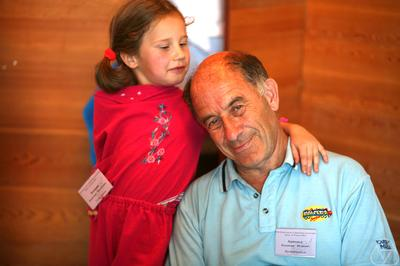
\includegraphics[width=\linewidth]{resources/photo-arnold_small}
}
\date{}

\begin{document}

\maketitle
\thispagestyle{empty}
\cleardoublepage
\setcounter{page}{1}

\begin{abstract}
Dit boek bevat 78 opgaven ter bevordering van een denkcultuur, uitgekozen of bedacht door de auteur. De meeste vergen geen bijzondere voorkennis anders dan algemeen onderwijs, maar som\-mige kunnen zelfs voor hoogleraren uitdagend zijn.

Het boek richt zich tot scholieren, studenten, leerkrachten, ouders -- tot allen die een denkcultuur als een wezenlijk onderdeel van de persoonlijke ontwikkeling beschouwen.
\end{abstract}

\cleardoublepage

\section*{Voorwoord}
Ik heb deze opgaven opgeschreven in Parijs in het voorjaar van 2004, toen Russische inwoners van Parijs me vroegen hun jonge kinderen te helpen de denkcultuur te verwerven die traditioneel is voor Rusland en die uitstijgt boven denkgewoonten in het Westen.

Ik ben er ten diepste van overtuigd dat deze cultuur het beste wordt ontwikkeld door het vroeg en zelfstandig nadenken over opgaven die eenvoudig op te schrijven maar moeilijk op te lossen zijn, zoals die hieronder (ik beveel vooral de opgaven~1, 3 en 13 aan).

Mijn lange ervaring heeft me duidelijk gemaakt dat matige leer\-lingen, die op school achterblijven, ze vaak beter oplossen dan uit\-blinkende leerlingen, omdat zij -- om achter in de klas te overleven~-- handiger moeten kunnen nadenken dan nodig om ``heel Sevilla en Granada te regeren'', zoals Figaro over zichzelf zei, terwijl toppers zich bij deze opgaven verliezen in ``wat met wat moet worden vermenig\-vuldigd''. Ik heb zelfs ontdekt dat kinderen van vijf jaar oud zulke opgaven beter oplossen dan schoolkinderen verpest door begeleiding, die op hun beurt de vragen beter aankunnen dan gedrilde studenten, die weer hun hoogleraren verslaan (het allerslechtst in het oplossen van deze opgaven zijn winnaars van de Nobelprijs of de Fieldsmedaille).

\clearpage

\section*{Opmerkingen bij de Duitse uitgave}
We hebben de vrijheid genomen bepaalde opgaven in het laatste deel van het boek van aanwijzingen en een nieuwe afbeelding te voorzien, en in vergelijking met de Engelse vertaling ook anders te verwoorden. Dit betreft de volgende opgaven: 52 (vrijer verwoord), 61 (aanwijzing toegevoegd), 64 (vrijer verwoord), 74 (afbeelding en uitleg toegevoegd), 75--77 (uitleg toegevoegd).

Verder hebben we aan het eind van het boek een korte verklarende woordenlijst opgenomen met definities van in het boek gebruikte wis\-kundige begrippen.

We stellen het op prijs reacties op de opgaven te ontvangen, om het gebruik van dit boek te verbeteren. Deze mogen uiteenlopen van oplossingsvoorstellen voor de opgaven, uitbreidingen van de verkla\-rende woordenlijst en nieuwe vertalingen, tot ideeën voor andere ver\-woordingen van de opgaven en aanvullende uitleg. Reacties, op- en aanmerkingen en verbetervoorstellen graag richten aan:\\\href{mailto:info@imaginary.org}{\nolinkurl{info@imaginary.org}}.

\section*{Opmerkingen bij de Nederlandse uitgave}
V.\,I.~Arnold heeft de originele uitgave van dit boek geschreven in het Russisch. Uw dienaar is die taal niet machtig en heeft zich voor deze Nederlandse uitgave op de Engelse en Duitse IMAGINARY vertalin\-gen verlaten. De Duitse uitgave, gebaseerd op de Engelse vertaling van het origineel, bevat een aantal eigen toevoegingen. Die zijn in deze Nederlandse uitgave meegenomen.

Ook geraadpleegd is de Nederlandse Google Translate vertaling van het Russische origineel; die gaf weliswaar nauwelijks nette zinnen, maar wel hier en daar treffende woorden.

Dit basismateriaal inspireerde een veelheid aan vertaalmogelijk\-heden. Er is voor gekozen de gebalde stijl van Arnold aan te houden.

\clearpage

\section*{De opgaven}

\begin{problem}{1.}
	Masha kwam zeven kopeken tekort om een leesboek te kopen, en Misha had één kopeke te weinig. Ze legden hun geld bij elkaar om het boek samen te kopen, maar zelfs toen hadden ze nog niet genoeg. Hoeveel kostte het boek?
\end{problem}

\begin{problem}{2.}
	Een fles met een kurk kost 10 kopeken, terwijl de fles alleen 9~kopeken duurder is dan de kurk. Hoeveel kost de fles zonder de kurk?
\end{problem}

\begin{problem}{3.}
	Een baksteen weegt een pond plus een halve steen. Hoeveel weegt de baksteen?
\end{problem}

\begin{problem}{4.}
	Een lepel wijn wordt vanuit een wijnvat in een (niet volledig gevuld) glas thee gegoten. Vervolgens wordt er een even grote lepel van het (inhomogene) mengsel vanuit het glas in het vat teruggebracht. Nu zit er zowel in het vat als in het glas een zekere hoeveelheid vreemde vloeistof (wijn in het glas en thee in het vat). Waarin is het volume vreemde vloeistof het grootst: in het glas of in het vat?
\end{problem}

\begin{problem}{5.}
	Twee oude dames vertrokken tegelijkertijd, bij zonsopkomst, de ene van $A$ naar $B$ en de andere van $B$ naar $A$. Ze liepen elkaar op dezelfde weg tegemoet. Ze ontmoetten elkaar op het middaguur, stopten echter niet, en elk ging in hetzelfde tempo door. De eerste dame kwam aan in $B$ om \SI{16}{\uur} en de tweede bereikte $A$ om \SI{21}{\uur}. Hoe laat was de zonsopgang die dag?
\end{problem}

\begin{problem}{6.}
	Een opgave in een standaard Amerikaans examen luidt: De schui\-ne zijde (hypotenusa) van een rechthoekige driehoek is 10 inch lang en de hoogte van de driehoek vanaf de schuine zijde is 6 inch. Bepaal de oppervlakte van de driehoek.

	Scholieren in de Verenigde Staten hadden gedurende meer dan een decennium geen probleem met deze vraag. Toen kwam er een aantal Russische schoolkinderen uit Moskou en geen van hen kon een oplossing geven, in tegenstelling tot hun Amerikaanse evenknieën (die als antwoord 30 vierkante inch gaven). Waarom?
\end{problem}

\begin{problem}{7.}
	Vasya heeft 2 zussen meer dan dat hij broers heeft. Hoeveel meer dochters dan zonen hebben Vasya's ouders?
\end{problem}

\clearpage

\begin{problem}{8.}
	Er is een ronde vijver in Zuid-Amerika, in het midden waarvan ieder jaar op 1~juni een Victoria Regia bloem verschijnt. De steel groeit vanuit de bodem en de bloembladen liggen op het wateroppervlak net zoals die van een waterlelie. Elke dag verdubbelt de oppervlakte van de bloem zich, totdat de bloembladen op 1~juli het gehele oppervlak van de vijver bedekken. Vervolgens vallen de bloembladen af en zinken de zaden naar de bodem. Op welke dag heeft de bloem de helft van de vijver bedekt?
\end{problem}

\begin{problem}{9.}
	Een boer moet een wolf, een geit en een kool met een boot een rivier overzetten. De boot is echter zo klein dat hij slechts één van de drie aan boord kan meenemen. Hoe kan hij alle drie de rivier overbrengen? (De wolf kan niet alleen gelaten worden met de geit, en de geit kan niet alleen gelaten worden met de kool.)
\end{problem}

\begin{problem}{10.}
	Overdag klimt een slak \SI{3}{\cm} tegen een paal omhoog, maar hij glijdt 's~nachts in zijn slaap weer \SI{2}{\cm} naar beneden. De paal is \SI{10}{\metre} hoog en helemaal bovenop bevindt zich een lekker hapje. Na hoeveel dagen zal de slak het hapje bereiken?
\end{problem}

\begin{problem}{11.}
	Een natuurbeheerder liep vanaf zijn tent \SI{10}{\km} zuidwaarts, sloeg af naar het oosten, liep \SI{10}{\km} oostwaarts, kwam zijn vriend de beer tegen, sloeg af naar het noorden, en kwam na nog eens \SI{10}{\km} weer bij zijn tent uit. Welke kleur had de beer, en waar gebeurde dit allemaal?
\end{problem}

\begin{problem}{12.}
	Het was vandaag om \SI{12}{\uur} 's~middags laagtij. Hoe laat zal dat morgen gebeuren (op dezelfde plaats)?
\end{problem}

\begin{problem}{13.}
	Twee van de werken van Poesjkin, het eerste en het tweede deel, staan naast elkaar op een boekenplank. De bladzijden van elk deel zijn samen \SI{2}{\cm} dik en de kaft, voorkaft en achterkaft elk, is \SI{2}{\mm} dik. Een boekenworm heeft zich doorgevreten, loodrecht op de bladzijden, van de eerste bladzijde van het eerste deel tot de laatste bladzijde van het tweede deel. Hoe lang is het gaatje?

	[Dit topologische vraagstuk met een onaannemelijk antwoord, te weten \SI{4}{\mm}, is onneembaar voor veel academici, terwijl sommige kleu\-ters er geen moeite mee hebben.]
\end{problem}

\clearpage

\begin{problem}{14.}
	Bedenk een lichaam met bovenaanzicht en vooraanzicht zoals hieronder getoond. Teken het zijaanzicht (duid onzichtbare ribben aan met een stippellijn).
	\begin{figure}
		\footnotesize
		\null\hfill
		\parbox{0.2\linewidth}{\centering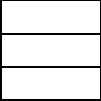
\includegraphics{resources/taskbook-99}\\Bovenaanzicht}
		\hfill
		\parbox{0.2\linewidth}{\centering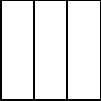
\includegraphics{resources/taskbook-98}\\Vooraanzicht}
		\hfill\null
	\end{figure}
\end{problem}

\begin{problem}{15.}
	Hoeveel manieren zijn er om het getal 64 te schrijven als de som van 10 natuurlijke getallen (gehele getallen $\geq 1$), waarvan er minstens één gelijk is aan en geen groter is dan 12?

	[Sommen die alleen verschillen in de volgorde van hun termen tellen niet als verschillend.]
\end{problem}

\begin{problem}{16.}
	Door gelijke staven (bijvoorbeeld dominostenen) op elkaar te stapelen, kunnen we de hoogste laten uitsteken over de laagste met een lengte van $x$ maal de staaflengte. Wat is de hoogst haalbare waarde van $x$?
	\begin{figure}
		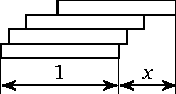
\includegraphics{resources/taskbook-97}
	\end{figure}
\end{problem}

\begin{problem}{17.}
	De afstand tussen twee steden $A$ en $B$ is \SI{40}{\km}. Twee fietsers vertrekken gelijktijdig uit $A$ en $B$ en rijden elkaar tegemoet, de ene met een snelheid van \SI{10}{\km\per\uur} en de andere met \SI{15}{\km\per\uur}. Een vlieg gaat met \SI{100}{\km\per\uur} tegelijk met de eerste fietser weg uit $A$, bereikt de tweede fietser, raakt zijn voorhoofd, vliegt terug naar de eerste fietser, raakt diens voorhoofd, dan weer terug naar de tweede en zo verder, totdat de voorhoofden van de fietsers elkaar raken en de vlieg wordt geplet. Hoeveel kilometer heeft de vlieg in totaal afgelegd?
	\begin{figure}
		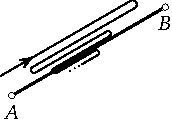
\includegraphics{resources/taskbook-1}
	\end{figure}
\end{problem}

\clearpage

\begin{problem}{18.}
	Een dominosteen bedekt steeds precies twee velden van een schaakbord. Probeer het gehele bord, behalve twee tegenoverliggende hoekvelden (op dezelfde diagonaal), te bedekken met 31 stenen. [Een schaakbord bestaat uit $8 \times 8 = 64$ vierkante velden.]
	\begin{figure}
		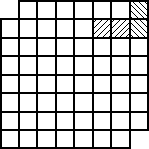
\includegraphics{resources/taskbook-2}
	\end{figure}
\end{problem}

\begin{problem}{19.}
	Een rups wil in een kubusvormige kamer van een hoek (linksvoor op de vloer) naar de tegenoverliggende hoek (rechtsachter tegen het plafond) kruipen. Bepaal de kortst mogelijke weg langs de wanden.
	\begin{figure}
		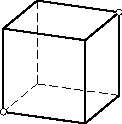
\includegraphics{resources/taskbook-3}
	\end{figure}
\end{problem}

\begin{problem}{20.}
	Je hebt twee vaten, het ene met een inhoud van 5 liter en het andere 3 liter, en water uit de kraan. Meet een liter af (overblijvend in één van beide vaten).
	\begin{figure}
		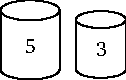
\includegraphics{resources/taskbook-4}
	\end{figure}
\end{problem}

\begin{problem}{21.}
	In een gezin zijn er vijf hoofden en veertien benen. Hoeveel mensen en hoeveel honden telt het gezin?
\end{problem}

\clearpage

\begin{problem}{22.}
	Op de zijden $AB$, $BC$ en $CA$ van een driehoek $ABC$ worden naar buiten toe gelijkzijdige driehoeken geconstrueerd. Bewijs dat hun centra (in de figuur aangegeven met $*$) een gelijkzijdige driehoek bepalen.
	\begin{figure}
		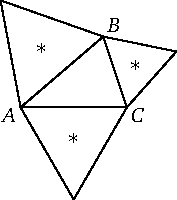
\includegraphics{resources/taskbook-6}
	\end{figure}
\end{problem}

\begin{problem}{23.}
	Welke veelhoeken kunnen ontstaan als een plat vlak een kubus doorsnijdt? Kunnen we zo een vijfhoek (pentagon), een zevenhoek (heptagon), een regelmatige zeshoek (hexagon) verkrijgen?
	\begin{figure}
		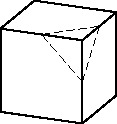
\includegraphics{resources/taskbook-7}
	\end{figure}
\end{problem}

\begin{problem}{24.}
	Teken een rechte lijn door het middelpunt van een kubus, zodat de som van de kwadraten van de afstanden ernaartoe vanuit de acht hoekpunten van de kubus a) zo groot mogelijk en b) zo klein mogelijk is (vergeleken met andere rechten door het midden).
\end{problem}

\clearpage

\begin{problem}{25.}
	Een rechtopstaande kegel met als basis een cirkel wordt door\-sneden door een plat vlak langs een gesloten kromme. Twee bollen die in de kegel zijn bevat raken het vlak, de ene in een punt $A$ en de andere in een punt $B$. Bepaal een punt $C$ op de snijkromme, waarvoor de som van de afstanden $CA + CB$ a) zo groot mogelijk en b) zo klein mogelijk is.
	\begin{figure}
		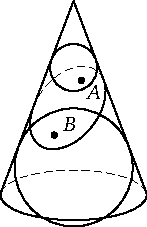
\includegraphics{resources/taskbook-9}
	\end{figure}
\end{problem}

\begin{problem}{26.}
	Het aardoppervlak wordt geprojecteerd op de cylinder gevormd door de raaklijnen aan de meridianen in de punten waar ze de evenaar snijden. De projectie verloopt langs de stralen door de aardas en evenwijdig aan het vlak van de evenaar. Is de oppervlakte van de projectie van Frankrijk groter of kleiner dan de werkelijke oppervlakte van Frankrijk?
	\begin{figure}
		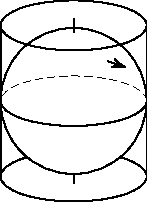
\includegraphics{resources/taskbook-10}
	\end{figure}
\end{problem}

\begin{problem}{27.}
	Bewijs dat voor een oneven priemgetal $p$ het delen van het getal~$2^{p-1}$ door $p$ een rest van 1 geeft (voorbeelden: $2^2 = 3 a + 1$, $2^4 = 5 b + 1$, $2^6 = 7 c + 1$, $2^{10} - 1 = 1023 = 11 \cdot 93$).
\end{problem}

\clearpage

\begin{problem}{28.}
	Een naald van \SI{10}{\cm} lang wordt willekeurig op een vel gelinieerd papier geworpen, waarvan de regelafstand ook \SI{10}{\cm} bedraagt. Dit wordt $N$ (zeg een miljoen) maal herhaald. Hoe vaak (ongeveer, met een fout van hoogstens een paar procent) kruist de gevallen naald een lijn op het papier?
	\begin{figure}
		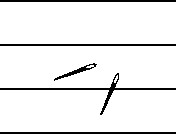
\includegraphics{resources/taskbook-12}
	\end{figure}
	Het is mogelijk dit experiment uit te voeren met slechts $N = 100$ (zoals ik deed toen ik 10 jaar oud was) in plaats van een miljoen maal. [Het antwoord op deze vraag is verrassend: $\frac{2}{\pi} N$. Zelfs voor een gebogen naald ter lengte $a \cdot \SI{10}{\cm}$ zal het aantal waargenomen treffers bij $N$ worpen bij benadering $\frac{2 a}{\pi} N$ zijn. Het getal $\pi \approx \frac{355}{113} \approx \frac{22}{7}$.]
\end{problem}

\begin{problem}{29.}
	Sommige veelvlakken hebben enkel driehoekige zijvlakken, zoals de volgende Platonische lichamen (regelmatige veelvlakken): tetraëder (4 zijvlakken), octaëder (8 zijvlakken), icosaëder (20 zijvlakken, met 12 hoekpunten en 30 ribben; is interessant om te tekenen).
	\begin{figure}
		\footnotesize
		\null\hfill
		\parbox{0.3\linewidth}{\centering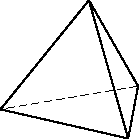
\includegraphics{resources/taskbook-131}\\Tetraëder ($\text{tetra} = 4$)}
		\hfill
		\parbox{0.3\linewidth}{\centering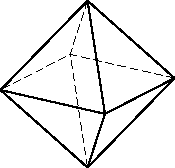
\includegraphics{resources/taskbook-132}\\Octaëder ($\text{octo} = 8$)}
		\hfill\null\\
		{\Huge ?}\\Icosaëder ($\text{icosi} = 20$)
	\end{figure}
	Onderzoek de bewering dat van zo'n lichaam (een begrensd convex veelvlak met driehoekige zijvlakken) het aantal zijvlakken gelijk is aan tweemaal het aantal hoekpunten min vier.
\end{problem}

\clearpage

\noindent Nog een Platonisch lichaam (er zijn er maar 5):
\begin{figure}
	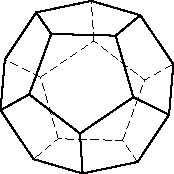
\includegraphics{resources/taskbook-14}
\end{figure}

\begin{problem}{30.}
	Een dodecaëder is een convex veelvlak met twaalf (regelmatige) vijfhoekige zijvlakken, twintig hoekpunten en dertig ribben; de hoek\-punten bevinden zich steeds in het midden van de zijvlakken van een icosaëder.

	Zoek vijf verschillende kubussen in het inwendige van de dode\-caëder, die voldoen aan de volgende eigenschappen: de hoekpunten van elke kubus zijn ook hoekpunten van de dodecaëder, en de ribben van elke kubus zijn diagonalen van de zijvlakken van de dodecaëder; bedenk dat een kubus 12 ribben heeft, één per zijvlak van de dodecaë\-der. [Johannes Kepler wierp deze constructie op in zijn model van de planetenbanen.]
\end{problem}

\begin{problem}{31.}
	Bepaal de doorsnede van twee tetraëders die zodanig in een kubus liggen, dat hun hoekpunten ook hoekpunten van de kubus zijn, en hun ribben diagonalen van zijvlakken van de kubus.

	Welk breukdeel van de kubusinhoud maakt de doorsnede van de tetraëders uit?
\end{problem}

\begin{problem}{31\textsuperscript{bis}.}
	Construeer de doorsnede van een kubus en een plat vlak dat door drie gegeven punten op de ribben van de kubus gaat (zie teke\-ning). [Teken de veelhoek die de doorsnede vormt van het vlak en de zijden van de kubus.]
	\begin{figure}
		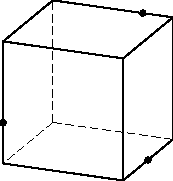
\includegraphics{resources/taskbook-15}
	\end{figure}
\end{problem}

\clearpage

\begin{problem}{32.}
	Hoeveel symmetrieën heeft een tetraëder? Hoeveel een kubus? Een octaëder? Een icosaëder? Een dodecaëder? Een symmetrie is een omzetting die een voorwerp op zichzelf afbeeldt, dus in het bijzonder de afmetingen van het voorwerp bewaart.

	Hoeveel van de symmetrieën zijn draaiingen (rotaties) en hoeveel ervan zijn spiegelingen (reflecties) (in elk van de vijf gevallen)?
\end{problem}

\begin{problem}{33.}
	Hoeveel manieren zijn er om de 6 zijvlakken van even grote kubussen in zes verschillende kleuren $(1,\dotsc,6)$ [één kleur per zijvlak] te verven, zodat er geen twee van de zo verkregen gekleurde kubussen gelijk zijn (geen twee kunnen door een draaiing in elkaar overgevoerd worden)?
	\begin{figure}
		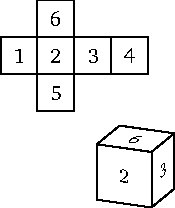
\includegraphics{resources/taskbook-17}
	\end{figure}
\end{problem}

\begin{problem}{34.}
	Hoeveel verschillende manieren zijn er om $n$ voorwerpen te rang\-schikken? Voor $n = 3$ zijn dat er zes: $(1,2,3)$, $(1,3,2)$, $(2,1,3)$, $(2,3,1)$, $(3,1,2)$, $(3,2,1)$. En hoeveel voor $n = 4$? $n = 5$? $n = 6$? $n = 10$?
	\begin{figure}
		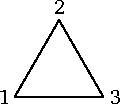
\includegraphics{resources/taskbook-18}
	\end{figure}
\end{problem}

\clearpage

\begin{problem}{35.}
	Een kubus heeft 4 lichaamsdiagonalen. Hoeveel permutaties van deze diagonalen zijn te verkrijgen via draaiingen van de kubus?
	\begin{figure}
		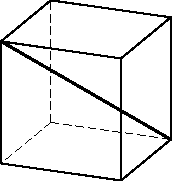
\includegraphics{resources/taskbook-19}
	\end{figure}
\end{problem}

\begin{problem}{36.}
	De som van de derdemachten van een aantal gehele getallen wordt afgetrokken van de derdemacht van de som van deze getallen. Is dit verschil altijd deelbaar door 3?
\end{problem}

\begin{problem}{37.}
	Dezelfde opgave als de vorige, maar dan voor de vijfde machten en deelbaarheid door 5, en voor de zevende machten en deelbaarheid door 7.
\end{problem}

\begin{problem}{38.}
	Bereken de som
	\begin{equation*}
		\frac{1}{1 \cdot 2} + \frac{1}{2 \cdot 3} + \frac{1}{3 \cdot 4} + \dotsb + \frac{1}{99 \cdot 100}
	\end{equation*}
	(de fout mag niet groter zijn dan $1\%$ van het antwoord).
\end{problem}

\begin{problem}{39.}
	Als twee verschillende veelhoeken dezelfde oppervlakte hebben, dan kunnen ze in een eindig aantal veelhoekjes worden verdeeld, die zo kunnen worden gelegd dat ze elk van beide veelhoeken vormen. Bewijs dit. [Voor driedimensionale lichamen geldt dit niet: een kubus en een tetraëder met dezelfde inhoud kunnen niet zodanig worden opgedeeld!]
	\begin{figure}
		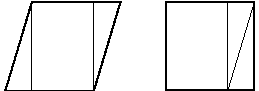
\includegraphics{resources/q39_horizontal}
	\end{figure}
\end{problem}

\clearpage

\begin{problem}{40.}
	Een parallellogram getekend op een vel ruitjespapier heeft zijn hoekpunten op roosterpunten. Verder liggen er noch op de zijden van het parallellogram noch in zijn binnengebied andere roosterpunten. Bewijs dat de oppervlakte van zo'n parallellogram gelijk is aan die van één ruitje.
	\begin{figure}
		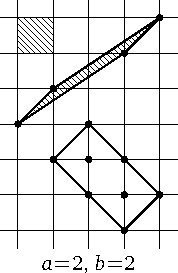
\includegraphics{resources/taskbook-24}
	\end{figure}
\end{problem}

\begin{problem}{41.}
	Met hetzelfde uitgangspunt als in opgave~40 liggen er nu $a$~roos\-terpunten binnen het parallellogram en $b$ op de zijden. Bereken zijn oppervlakte.
\end{problem}

\begin{problem}{42.}
	Geldt voor parallellepipeda in de ruimte de overeenkomstige uitspraak uit opgave~40 ook?
\end{problem}

\begin{problem}{43.}
	De Fibonacci-getallen vormen de rij $1,1,2,3,5,8,13,21,34,\dotsc$ (de rij van Fibonacci of ook wel de konijnenrij genoemd), waarin geldt: $a_1 = 1$, $a_2 = 1$, $a_{n+2} = a_{n+1} + a_n$ voor alle $n = 1,2,\dotsc$ ($a_n$ is het $n$de~getal in de rij). Bepaal de grootste gemene deler van de getallen $a_{100}$ en $a_{99}$.
\end{problem}

\clearpage

\begin{problem}{44.}
	Bepaal het aantal manieren (Catalan-getal $c(n)$) om een convexe $n$-hoek in driehoeken te verdelen door te knippen langs diagonalen die elkaar niet snijden. Bijvoorbeeld $c(4) = 2$, $c(5) = 5$, $c(6) = 14$. Hoe bepaal je $c(10)$?
	\begin{figure}
		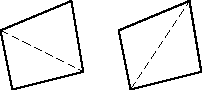
\includegraphics{resources/taskbook-281}
		\qquad
		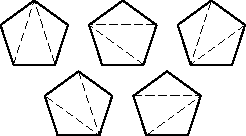
\includegraphics{resources/taskbook-282}
	\end{figure}
\end{problem}

\begin{problem}{45.}
	Aan een toernooi doen $n$ ploegen mee. Een ploeg die verliest valt af. Dus na $n - 1$ partijen blijft de winnaar over. Het wedstrijdschema voor vier ploegen kan worden geschreven met een symbool:\\$((a,(b,c)),d)$ betekent dat eerst de ploegen $b$ en $c$ tegen elkaar uit\-komen, de winnaar dan tegen $a$ speelt, en de winnaar van die partij ten slotte tegen $d$. Hoeveel verschillende schema's zijn er voor 10 ploegen?
	\begin{itemize}
		\item Bij 2 ploegen is er alleen de mogelijkheid $(a,b)$, aantal = 1.
		\item Bij 3 ploegen zijn er de mogelijkheden $((a,b),c)$, $((a,c),b)$, $((b,c),a)$, aantal = 3.
		\item Bij 4 ploegen zijn er de volgende, aantal = 15:
		    \begin{equation*}
	    	\begin{array}{@{}cccc@{}}
	    	(((a,b),c),d) & \quad\;(((a,c),b),d) & \quad\;(((a,d),b),c) & \quad\;(((b,c),a),d) \\
	    	(((b,d),a),c) & \quad\;(((c,d),a),b) & \quad\;(((a,b),d),c) & \quad\;(((a,c),d),b) \\
	    	(((a,d),c),b) & \quad\;(((b,c),d),a) & \quad\;(((b,d),c),a) & \quad\;(((c,d),b),a) \\
	    	((a,b),(c,d)) & \quad\;((a,c),(b,d)) & \quad\;((a,d),(b,c))
	    	\end{array}
	    	\end{equation*}
	\end{itemize}
\end{problem}

\begin{problem}{46.}
	Verbind $n$ punten $1,2,\dotsc,n$ met $n - 1$ lijnstukken tot een boom. Hoeveel verschillende bomen kun je vormen? (Het geval $n = 5$ is al interessant!)

	$n = 2$:\quad
    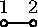
\includegraphics{resources/taskbook-291}\,,\quad
    aantal = 1;

	$n = 3$:\quad
	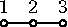
\includegraphics{resources/taskbook-292}\,,\quad
	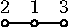
\includegraphics{resources/taskbook-293}\,,\quad
	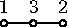
\includegraphics{resources/taskbook-294}\,,\quad
	aantal = 3;

	$n = 4$:\quad
	$\vcenter{\hbox{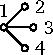
\includegraphics{resources/taskbook-295}}}$,\quad
	$\vcenter{\hbox{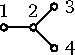
\includegraphics{resources/taskbook-296}}}$,\quad
	$\vcenter{\hbox{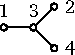
\includegraphics{resources/taskbook-297}}}$,\quad
	$\vcenter{\hbox{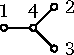
\includegraphics{resources/taskbook-298}}}$,\quad
	$\vcenter{\hbox{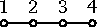
\includegraphics{resources/taskbook-299}}\hbox{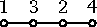
\includegraphics{resources/taskbook-290}}
	\vskip-8pt
	\hbox to50bp{\dotfill}}$,\\
	\null\hspace{\parindent}\phantom{$n = 4$:}\quad
    aantal = 16.
\end{problem}

\clearpage

\begin{problem}{47.}
	Een permutatie $(x_1,x_2,\dotsc,x_n)$ van de getallen $\{1,2,\dotsc,n\}$ heet een `slang' (ter lengte $n$) als $x_1 < x_2 > x_3 < x_4 \dotsb$.\\

\noindent \texttt{Voorbeeld}
	\begin{equation*}
	\begin{aligned}[t]
	&\begin{aligned}[t] n=2, \text{\ \ alleen\ \ } 1<2, \end{aligned} && \text{aantal} = 1, \\
	&\hskip-\nulldelimiterspace\mathord{\left. \begin{aligned} n=3, \hphantom{\text{\ \ alleen\ \ }} 1&<3>2 \\
	2&<3>1 \end{aligned} \right\}}, && \text{aantal} = 2, \\
	&\hskip-\nulldelimiterspace\mathord{\left. \begin{aligned} n=4, \hphantom{\text{\ \ alleen\ \ }} 1&<3>2<4 \\
	1&<4>2<3 \\
	2&<3>1<4 \\
	2&<4>1<3 \\
	3&<4>1<2 \end{aligned} \right\}},
	&& \text{aantal} = 5. \\
	\end{aligned}
	\end{equation*}

	Bepaal het aantal slangen ter lengte 10.
\end{problem}

\begin{problem}{48.}
	Laat $s_n$ het aantal slangen ter lengte $n$ aangeven:
	\begin{equation*}
		s_1 = 1, \quad s_2 = 1, \quad s_3 = 2, \quad s_4 = 5, \quad s_5 = 16, \quad s_6 = 61.
	\end{equation*}
	Toon aan dat de Taylorreeks van de tangensfunctie luidt
	\begin{equation*}
		\tan x = 1\, \frac{x^1}{1!} + 2\, \frac{x^3}{3!} + 16\, \frac{x^5}{5!} + \dots = \textstyle\sum\limits_{k=1}^{\infty} s_{2k - 1}\, \frac{x^{2k - 1}}{(2k - 1)!}.
	\end{equation*}
\end{problem}

\begin{problem}{49.}
	Bepaal de som van de reeks
	\begin{equation*}
		1 + 1\, \frac{x^2}{2!} + 5\, \frac{x^4}{4!} + 61\, \frac{x^6}{6!} + \dots = \textstyle\sum\limits_{k=0}^{\infty} s_{2k}\, \frac{x^{2k}}{(2k)!}.
	\end{equation*}
\end{problem}

\begin{problem}{50.}
	Bewijs voor $s > 1$ de gelijkheid
	\begin{equation*}
		\textstyle\prod\limits_{p=2}^{\infty} \frac{1}{1 - \frac{1}{p^s}} = \textstyle\sum\limits_{n=1}^{\infty} \frac{1}{n^s}
	\end{equation*}
	(het product loopt over alle priemgetallen $p$, de som over alle natuur\-lijke getallen $n$).
\end{problem}

\clearpage

\begin{problem}{51.}
	Bepaal de som van de reeks
	\begin{equation*}
		1 + \frac{1}{4} + \frac{1}{9} + \dots = \textstyle\sum\limits_{n=1}^{\infty} \frac{1}{n^2}
	\end{equation*}
	(bewijs dat deze gelijk is aan $\nicefrac{\pi^2}{6}$, dus bij benadering $\nicefrac{3}{2}$).
\end{problem}

\begin{problem}{52.}
	$R$ is de straal van een cirkelschijf, en $p$ en $q$ zijn twee gehele getallen die voldoen aan de ongelijkheid $p^2 + q^2 \leqslant R^2$. Hoe groot is de kans dat de breuk $\nicefrac{p}{q}$ niet meer kan worden vereenvoudigd?

	We tellen op de cirkelschijf de punten waarvan de coördinaten onderling ondeelbare gehele getallen zijn (geen gemene deler anders dan 1). We noemen dit aantal $N(R)$ (het aantal punten $N$ hangt af van de straal $R$; dat maken we in de notatie $N(R)$ duidelijk). Verder is $M(R)$ het aantal punten op de cirkelschijf met geheeltallige coördinaten ($M(R) \sim \pi R^2$). De kans dat de breuk $\nicefrac{p}{q}$ niet meer kan worden vereenvoudigd is dan de limiet van de breuk $\nicefrac{N(R)}{M(R)}$.
	\begin{figure}
		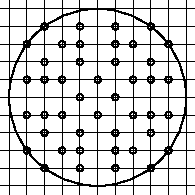
\includegraphics{resources/taskbook-36}\\
		\footnotesize $M(5) = 81,N(5) = 44,\nicefrac{N}{M} = \nicefrac{44}{81}$
	\end{figure}
\end{problem}

\clearpage

\begin{problem}{53.}
	Bepaal voor de rij Fibonacci-getallen $a_n$ uit opgave~43 de limiet van de verhouding $a_{n+1}/a_n$ wanneer $n$ naar oneindig gaat:
	\begin{equation*}
		\frac{a_{n+1}}{a_n} = 1, \ 2, \ \frac{3}{2}, \ \frac{5}{3}, \ \frac{8}{5}, \ \frac{13}{8}, \ \frac{21}{13}, \ \frac{34}{21}, \ \dotsc
	\end{equation*}
\noindent \texttt{Antwoord:} De `gulden snede', $\frac{\sqrt{5} + 1}{2} \approx 1{,}618$. [Deze is de verhouding tussen de zijden van een rechthoek $ABCD$ die gelijkvormig is aan wat er overblijft na afsnijden van het vierkant $ABPQ$ met als zijde de korte zijde van de rechthoek, $\frac{AB}{BC} = \frac{PC}{CD}$.] Hoe treedt de gulden snede op in een regelmatige vijfhoek (pentagon) en een vijfpuntige ster (pentagram)?
	\begin{figure}
		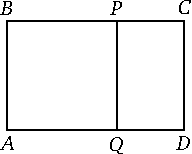
\includegraphics{resources/taskbook-37}
	\end{figure}
\end{problem}

\begin{problem}{54.}
	Bereken de waarde van de oneindige kettingbreuk
	\begin{equation*}
		1 + \cfrac{1}{2 + \cfrac{1}{1 + \cfrac{1}{2 + \cfrac{1}{1 + \cfrac{1}{2 + \ldots}}}}} = a_0 + \cfrac{1}{a_1 + \cfrac{1}{a_2 + \cfrac{1}{a_3 + \ldots}}}
	\end{equation*}
	met $a_{2k} = 1$ en $a_{2k + 1} = 2$ (bepaal de limiet van de breuken
	\begin{equation*}
		a_0 + \cfrac{1}{a_1 + \cfrac{1}{a_2 + {\atop{\ddots\atop{}} + \cfrac{1}{a_n}}}}
	\end{equation*}
	voor $n \to \infty$).
\end{problem}

\clearpage

\begin{problem}{55.}
	Druk uit in veeltermen (polynomen)
	\begin{equation*}
		y = \cos (3 \arccos x),\ y = \cos (4 \arccos x),\ y = \cos (n \arccos x),
	\end{equation*}
	waarbij $|x| \leqslant 1$.
\end{problem}

\begin{problem}{56.}
	Bereken de som van de $k$de machten van de $n$ (complexe) $n$de eenheidswortels.
\end{problem}

\begin{problem}{57.}
	Teken in het $(x,y)$-vlak de krommen gedefinieerd door de para\-metervoorstellingen
	\begin{equation*}
		\{x = \cos 2 t, y = \sin 3 t\},\quad
		\{x = t^3 - 3 t, y = t^4 - 2 t^2\}.
	\end{equation*}
\end{problem}

\begin{problem}{58.}
	Bereken (de fout mag niet groter zijn dan $10\%$ van het antwoord)
	\begin{equation*}
		\int_{0}^{2 \pi} \sin^{100} x\,dx.
	\end{equation*}
\end{problem}

\begin{problem}{59.}
	Bereken (de fout mag niet groter zijn dan $10\%$ van het antwoord)
	\begin{equation*}
		\int_{1}^{10} x^x\,dx.
	\end{equation*}
\end{problem}

\begin{problem}{60.}
	Bepaal de oppervlakte $S$ van een driehoek met hoeken $(\alpha,\beta,\gamma)$ op een bol met straal 1, waarvan de zijden liggen op grootcirkels (doorsnedes van de bol met platte vlakken die door het middelpunt van de bol gaan).\\

\noindent \texttt{Antwoord:} $S = \alpha + \beta + \gamma - \pi$ (bijvoorbeeld voor een driehoek met drie rechte hoeken bedraagt $S = \nicefrac{\pi}{2}$, een achtste van de oppervlakte van de bol).
	\begin{figure}
		\null\hfill
		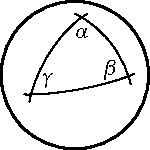
\includegraphics{resources/taskbook-44}
		\hfill\null
	\end{figure}
\end{problem}

\clearpage

\begin{problem}{61.}
	Een cirkel met straal $r$ rolt (zonder te slippen) binnen een cirkel met straal 1. Teken de volledige baan van een punt op de rollende cirkel (zo'n baan heet een hypercycloïde) voor $r = \nicefrac{1}{3}$, voor $r = \nicefrac{1}{4}$, voor $r = \nicefrac{1}{n}$, voor $r = \nicefrac{1}{2}$.\\

\noindent \texttt{Aanwijzing:} Voer dit gedachtenexperiment vervolgens uit op een over een rechte rollende cirkel. De resulterende kromme heet een cycloïde. Zet dit geval nu over naar de oorspronkelijke opgave.
	\begin{figure}
		\null\hfill
		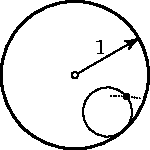
\includegraphics{resources/taskbook-45}
		\hfill\null
	\end{figure}
\end{problem}

\begin{problem}{62.}
	Hoe groot is de kans dat in een klas van $n$ leerlingen er twee op dezelfde dag jarig zijn? Vind je deze kans groot of klein?\\

\noindent \texttt{Antwoord:} (Zeer) groot als het leerlingenaantal $n$ (ver) boven een zekere $n_0$ ligt, (zeer) klein als het (ver) onder $n_0$ ligt, en wat deze opgave eigenlijk vraagt is welke waarde $n_0$ heeft (wanneer de kans ongeveer $\nicefrac{1}{2}$ is).
\end{problem}

\clearpage

\begin{problem}{63.}
	De brekingswet van Snellius zegt dat de hoek $\alpha$ tussen een lichtstraal en de loodlijn op het oppervlak van een gelaagd medium wordt bepaald door de vergelijking
	\begin{equation*}
		n(y) \sin \alpha = \text{constant},
	\end{equation*}
	waarbij $n(y)$ de brekingsindex van de laag ter hoogte $y$ is. (De index~$n$ is omgekeerd evenredig aan de lichtsnelheid in het medium, waarbij de snelheid in vacuüm op 1 wordt gesteld; in water is $n$ onafhankelijk van de hoogte $y$ en heeft de waarde $n = \nicefrac{4}{3}$.)
	\begin{figure}
		\null\hfill
		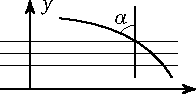
\includegraphics{resources/taskbook-47}
		\hfill\null
	\end{figure}

	Teken de banen van lichtstralen in het medium `lucht boven een woestijn', waarin de brekingsindex $n(y)$ op een bepaalde hoogte een maximum heeft:
	\begin{figure}
		\null\hfill
		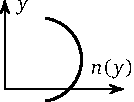
\includegraphics{resources/taskbook-471}
		\hfill\null
	\end{figure}

	(De oplossing van dit vraagstuk verklaart het verschijnsel van een luchtspiegeling in de woestijn, tenminste voor wie begrijpt hoe banen van lichtstralen afkomstig van een voorwerp in verband staan met het beeld ervan.)
\end{problem}

\clearpage

\begin{problem}{64.}
	Beschouw een scherphoekige driehoek $ABC$. Bepaal de driehoek $KLM$ met de kleinst mogelijke omtrek die zo in $ABC$ is ingeschreven dat de hoek $K$ op de zijde $AB$ ligt, $L$ op $BC$, en $M$ op $CA$.
	\begin{figure}
		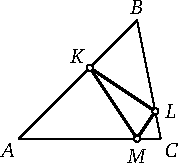
\includegraphics{resources/taskbook-48}
	\end{figure}
\noindent \texttt{Opmerking:} Voor niet-scherphoekige driehoeken is de oplossing niet zo elegant als voor scherphoekige.
\end{problem}

\begin{problem}{65.}
	Bereken het gemiddelde van de functie $\nicefrac{1}{r}$ ($r$ is de afstand van de oorsprong $(0,0,0)$ tot een willekeurig punt $(x,y,z)$, $r^2 = x^2 + y^2 + z^2$) op de bol met straal $R$ en middelpunt $(X,Y,Z)$.\\

\noindent \texttt{Opmerking:} Deze opgave staat in verband met de gravitatiewet van Newton en de wet van Coulomb uit de elektriciteitsleer. In de twee\-dimensionale versie van deze opgave dient de gegeven functie te wor\-den vervangen door $\ln r$ en de bol door een cirkel.
\end{problem}

\begin{problem}{66.}
	Uit het feit dat $2^{10} = 1024 \approx {10}^3$ volgt dat $\log_{10} 2 \approx 0,3$. Schat hun verschil en bereken $\log_{10} 2$ tot op drie decimalen nauwkeurig.
\end{problem}

\begin{problem}{67.}
	Bereken $\log_{10} 4$, $\log_{10} 8$, $\log_{10} 5$, $\log_{10} 50$, $\log_{10} 32$, $\log_{10} 128$,\\$\log_{10} 125$, $\log_{10} 64$ met dezelfde nauwkeurigheid.
\end{problem}

\begin{problem}{68.}
	Gebruik het feit dat $7^2 \approx 50$ om een benadering te bepalen van $\log_{10} 7$.
\end{problem}

\begin{problem}{69.}
	Bepaal $\log_{10} 9$, $\log_{10} 3$, $\log_{10} 27$, $\log_{10} 6$, $\log_{10} 12$, aannemende dat de waarden van $\log_{10} 64$ en $\log_{10} 7$ bekend zijn.
\end{problem}

\clearpage

\begin{problem}{70.}
	Bepaal, met gebruik van $\ln (1 + x) \approx x$ ($\ln$ staat voor $\log_e$)\footnote{Het getal van Euler $e = 2{,}71828 \dots$ is gedefinieerd als de limiet van de rij ${\left( 1 + \frac{1}{n} \right)}^n$ voor $n \to \infty$, en is gelijk aan de som van de reeks $1 + \frac{1}{1!} + \frac{1}{2!} + \frac{1}{3!} + \dotsb$. Het kan ook worden gedefinieerd via de aangehaalde formule voor $\ln (1 + x)$: $\lim\limits_{x \to 0} \frac{\ln (1 + x)}{x} = 1$.}, $\log_{10} e$ en $\ln 10$ uit de betrekking
	\begin{equation*}
		\log_{10} a = \frac{\ln a}{\ln 10}
	\end{equation*}
	en de eerder berekende waarden van $\log_{10} a$ (bijvoorbeeld voor $a = \nicefrac{128}{125},\nicefrac{1024}{1000}$ enzovoort).

	[De antwoorden uit de opgaven~66--70 leveren je, na een half uur rekenen, een logaritmetafel op in vier decimalen voor elk willekeurig getal, met behulp van producten van reeds als steunpunten gevonden getallen en met de formule
	\begin{equation*}
		\ln (1 + x) \approx x - \frac{x^2}{2} + \frac{x^3}{3} - \frac{x^4}{4} + \dotsb
	\end{equation*}
	ter correctie.] (Op deze manier stelde Newton een logaritmetafel op in 40 decimalen!)
\end{problem}

\begin{problem}{71.}
	Beschouw de rij machten van~2: $1,2,4,8,16,32,64,128,256,512,$\\$1024,2048,\dotsc$. Onder de eerste twaalf zijn er vier waarvan de decimale expansie begint met een 1, en geen waarvan deze begint met een 7.

	Bewijs dat in de limiet voor $n \to \infty$ het eerste cijfer van de getallen $2^m$, $0 \leqslant m \leqslant n$, voorkomt met een bepaalde frequentie: $p_1 \approx 30\%,p_2 \approx 18\%,\dotsc,p_9 \approx 4\%$.
\end{problem}

\begin{problem}{72.}
	Beschouw het gedrag van de eerste cijfers van de machten van~3: $1,3,9,2,8,2,7,\dotsc$. Bewijs dat voor dezelfde limiet als in opgave~71 ook bepaalde frequenties optreden, en wel dezelfde als voor de machten van~2. Bepaal een exacte formule voor $p_1,\dotsc,p_9$.\\

\noindent \texttt{Aanwijzing:} Het eerste cijfer van een getal $x$ wordt bepaald door het decimale deel van het getal $\log_{10} x$. Het volstaat dus de rij decimale delen van de getallen $m \alpha$ te beschouwen, waarbij $\alpha = \log_{10} 2$.

	Bewijs dat deze decimale delen gelijkmatig over het interval van 0 tot 1 verdeeld zijn: Voor een deelinterval $A$ van het interval van 0 tot 1 is $k_n(A)$ het aantal decimale delen van de $n$ getallen $m \alpha$, $0 \leqslant m < n$, die in $A$ liggen. Toon aan $\lim (k_n(A) / n) = (\text{Lengte deelinterval }A)$ voor $n \rightarrow \infty$.
\end{problem}

\clearpage

\begin{problem}{73.}
	Laat $M$ een begrensd domein zijn en $g \colon M \to M$ een gladde, injectieve afbeelding van $M$ in zichzelf die oppervlakten (volumes in het meerdimensionale geval) van gebieden bewaart.

	Beschouw een willekeurig punt in $M$ en een willekeurige omge\-ving~$U$ van dit punt. Neem verder een willekeurig natuurlijk getal $N$. Bewijs dat er een punt $x$ in $U$ bestaat, zodat voor een zeker natuurlijk getal $T \geq N$ geldt dat $g^T(x)$ weer in $U$ ligt (d.w.z. we beschouwen $g(g(\dots(x))$, waarbij $g$ in totaal $T$ maal wordt toegepast) (\textit{Terugkeer\-stelling van Poincaré}).
\end{problem}

\begin{problem}{74.}
	Laat $M$ het oppervlak van een torus aangeven (een torus ziet eruit als een donut). Men kan deze heel eenvoudig formeel beschrijven, wanneer men als coördinaat-assen deze twee cirkels kiest:
	\begin{figure}
		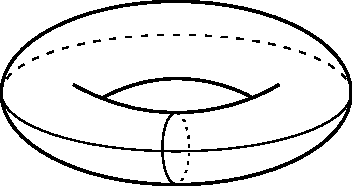
\includegraphics{resources/74_torus}
	\end{figure}
\noindent Punten met coördinaten $(a,0)$ liggen dan bijvoorbeeld op de horizon\-tale cirkel, punten met coördinaten $(0,b)$ op de vertikale. Omdat we na een volledige rondgang (${360}^\circ$ of $2 \pi$) langs elk van de cirkels weer in het vertrekpunt terugkomen, volstaat het de coördinaten modulo~$2 \pi$ te beschouwen.

	Laat de torus dus door de coördinaten ($\alpha$ mod $2 \pi$, $\beta$ mod $2 \pi$) beschreven zijn en $g \colon M \to M$ door
	\begin{equation*}
		g(\alpha,\beta) = (\alpha + 1,\beta + \sqrt{2}) \pmod {2 \pi}.
	\end{equation*}
	Toon aan dat de rij $\{g^T(x)\}$ voor alle $x$ op $M$ overal dicht in de torus ligt, waarbij $T$ de waarden $1,2,\dotsc$ doorloopt.
\end{problem}

\clearpage

\begin{problem}{75.}
	Laat met dezelfde uitgangspunten als in opgave~74 de afbeelding $g \colon M \to M$ gegeven zijn door
	\begin{equation*}
		g(\alpha,\beta) = (2 \alpha + \beta,\alpha + \beta) \pmod {2 \pi}.
	\end{equation*}
	Toon aan dat er een deelverzameling van de torus bestaat die overal dicht is en uit periodieke punten van $g$ bestaat. (`Periodiek' betekent dat $g^{T(x)}(x) = x$ geldt voor zekere natuurlijke getallen $T(x)$. Het getal~$T$ hangt hierbij af van het punt $x$; deze afhankelijkheid wordt in de notatie $T(x)$ uitgedrukt.)
\end{problem}

\begin{problem}{76.}
	We nemen dezelfde uitgangspunten als in opgave~74 en beschou\-wen de afbeelding uit opgave~75. Bewijs dat voor bijna alle punten $x$ op de torus de rij punten $\{g^T(x)\}$, $T = 1,2,\dotsc$, overal op de torus dicht is (`bijna alle' punten betekent dat de punten zonder deze eigenschap samen `maat', hier oppervlakte, nul hebben).
\end{problem}

\begin{problem}{77.}
	Bewijs in de opgaven~74 en 76 dat de rij $\{g^T(x)\}$, $T = 1,2,\dotsc$, gelijkmatig (uniform) over de torus verdeeld is. Hiermee wordt het volgende bedoeld: We beschouwen een deelverzameling $A$ van $M$, en tellen uit de eerste $n$ punten van de rij alleen de punten die in $A$ liggen. Dit aantal noemen we $k_n(A)$. Opdat de rij gelijkmatig verdeeld is, moet gelden
	\begin{equation*}
		\lim\limits_{n \to \infty} \frac{k_n(A)}{n} = \frac{\text{Oppervlakte}\,(A)}{\text{Oppervlakte}\,(M)}.
	\end{equation*}
\end{problem}

\vfill

\noindent \texttt{Opmerking bij opgave~13.} Met deze opgave probeerde ik in mijn bijdrage aan het 2000 milleniumnummer van het tijdschrift \textit{Physics -- Uspekhi} de verschillende probleembenaderingen die men doorgaans ziet bij wiskundigen en natuurkundigen te illustreren. Het succes over\-trof mijn verwachtingen. De redacteuren waren, in tegenstelling tot de kleuters op de ervaring met wie ik mijn plan baseerde, niet in staat het probleem op te lossen. Ze veranderden het als volgt om in hun ogen toe te werken naar mijn oplossing \SI{4}{\mm}: in plaats van ``van de eerste bladzijde van het eerste deel tot de laatste bladzijde van het tweede deel'' drukten ze af ``van de \textit{laatste} bladzijde van het eerste deel tot de \textit{eerste} bladzijde van het tweede deel''.

	Dit waargebeurde voorval is zo ongeloofwaardig dat ik het hier vermeld: het bewijs is de versie van de redactie zoals gepubliceerd in het tijdschrift.

\clearpage

\section*{Verklarende woordenlijst}

\begin{description}

	\item[Convex] Wiskundigen noemen een figuur (bijvoorbeeld een veelvlak) convex, als men tussen twee willekeurige punten van de figuur een rechte lijn kan tekenen en dat hele lijnstuk in het inwendige van de figuur ligt. Aanschouwelijk gesproken is een convexe fi\-guur overal bolstaand naar buiten.

	Voorbeelden:
	\begin{figure}
		\def\svgwidth{230pt}
		\subimport{resources/}{glossar_konvex.pdf_tex}
	\end{figure}

	\item[Dicht] Een deelverzameling $A$ van een `grote' verzameling $M$ ligt dicht in $M$, als men elk element van $M$ willekeurig goed kan benaderen met elementen uit $A$ (spreektaal: wanneer men met elementen uit $A$ willekeurig dicht bij elk element van $M$ kan komen).

	Bijvoorbeeld ligt de verzameling van de rationale getallen $\mathbb{Q}$ dicht in de verzameling van de reële getallen $\mathbb{R}$, d.w.z. elk reëel getal kan willekeurig goed door een breuk worden benaderd.

	\item[Eenheidswortel] Een $n$de eenheidswortel is een getal dat verheven tot de $n$de macht 1 oplevert (in formulevorm: een getal $z$ zodat $z^n = 1$).

	Bijvoorbeeld is 1 een $n$de eenheidswortel voor elk natuurlijk getal $n$, want er geldt $1^n = 1$. Als $n$ even is, is bovendien $-1$ een $n$de eenheidswortel, want dan geldt ${(-1)}^n = 1$.

	In het algemeen vindt men eenheidswortels op het terrein van de complexe getallen. Deze vormen het eersthogere getalbegrip boven de verzameling van de reële getallen $\mathbb{R}$. Het kan boeiend zijn je daar wat in te verdiepen.

\clearpage

	\item[Gladde afbeelding] Volgens de wiskundige definitie heet een afbeeld\-ing glad, als deze oneindig vaak differentieerbaar is. Bijvoorbeeld is elke veelterm (polynoom) glad:
	\begin{gather*}
		f(x) = x^2 + 3,\ f'(x) = 2 x,\ f''(x) = 2,\\
		f'''(x) = f^{(n)}(x) = 0 \text{ voor alle natuurlijke getallen } n \geq 3.
	\end{gather*}

	Ook de $e$-functie behoort tot de gladde afbeeldingen:
	\begin{equation*}
		g(x) = e^x, g'(x) = g^{(n)}(x) = e^x \text{ voor alle natuurlijke getallen } n.
	\end{equation*}

	Een voorbeeld van een functie die niet glad is, is de absolute waarde functie $h(x) = |x|$. Die heeft in $x = 0$ een `punt' en kan daar niet worden gedifferentieerd.

	Aanschouwelijk kan het woord `glad' bij functies letterlijk wor\-den opgevat: de grafiek van een gladde functie heeft geen punten en laat zich in één streek tekenen.

	\item[Injectief] Een afbeelding die geen element in het bereik meer dan eenmaal bereikt, heet injectief. Bijvoorbeeld is elke permutatie injectief (zie Permutatie).

	Voorbeelden:
	\begin{figure}
		\def\svgwidth{200pt}
		\subimport{resources/}{glossar_injektiv.pdf_tex}
	\end{figure}

	De functie $f(x) = x^2$ is niet injectief, wanneer men als domein de hele reële as toelaat. Dan is namelijk $f(-1) = f(1) = 1$, dus 1 wordt tweemaal bereikt.

	\item[Modulo] We schrijven $a \mod b$ en bedoelen de rest die overblijft als $a$ door $b$ wordt gedeeld. Vergelijkbaar met het gelijkheidsteken wordt in dit verband het symbool ``$\equiv$'' gebruikt.

	$c \equiv a \mod b$ (spreek uit: $c$ is congruent aan $a$ modulo $b$) be\-tekent dat $c$ en $a$ bij deling door $b$ dezelfde rest hebben.

	Voorbeelden: $7 \equiv 1 \mod 6,\ 11 \equiv 3 \mod 4$.

\clearpage

	\item[Permutatie] Een permutatie is een afbeelding, waarbij de getallen $1,2,\dotsc,n$ zodanig op de getallen $1,2,\dotsc,n$ worden afgebeeld, dat elk getal in het co-domein wordt bereikt.

	Voorbeelden:
	\begin{figure}
		\def\svgwidth{200pt}
		\subimport{resources/}{glossar_permutation.pdf_tex}
	\end{figure}

	\item[Productteken] Net als het somteken (zie Somteken) is het product\-teken $\prod$ een korte notatie voor ``deze getallen worden met elkaar vermenigvuldigd''. Ook hier worden de grenzen onder en boven het symbool geschreven.

	Voorbeelden:
	\begin{gather*}
		\prod\limits_{k=3}^{5} k = 3 \cdot 4 \cdot 5 = 60,\\
		\prod\limits_{m=4}^{7} (m^2 - m) = (4^2 - 4) \cdot (5^2 - 5) \cdot (6^2 - 6) \cdot (7^2 - 7) = 302\,400.
	\end{gather*}

\clearpage

	\item[Rij] Een rij is een opeenvolging van genummerde objecten, waaraan een voorschrift ten grondslag ligt. De rij zelf wordt als $(a_n) = a_1,a_2,a_3,\dotsc$ geschreven, het teken $a_n$ staat voor het $n$de~ele\-ment van de rij.

	Voorbeelden:
	\begin{itemize}
		\item De natuurlijke getallen met het voorschrift $a_n = n$:
		\begin{equation*}
			1,2,3,4,5,\dotsc{}
		\end{equation*}
		Men kan ook afzonderlijke elementen uit de rij lichten, bij\-voorbeeld $a_{14} = 14$.

		\item De Fibonacci-getallen met het voorschrift $a_{n+2} = a_{n+1} + a_n$ en de start $a_1 = a_2 = 1$:
		\begin{equation*}
			1,1,2,3,5,8,13,\dotsc{}
		\end{equation*}

		\item De rij die door het voorschrift $a_n = f^n(x)$ voor de functie $f(x) = 2 x - 1$ is gegeven. Hierbij hebben we natuurlijk een startwaarde voor $x$ nodig, bijvoorbeeld $x = 2$:
		\begin{equation*}
			a_1 = f(2) = 3,\ a_2 = f(3) = 5,\ a_3 = f(5) = 9,\dotsc
		\end{equation*}
		Anders geschreven luidt de rij aldus $3,5,9,17,33,\dotsc{}$
	\end{itemize}

	\item[Somteken] Het somteken $\sum$ is een korte notatie voor de uitspraak ``deze getallen worden bij elkaar opgeteld''. Opdat men weet van waar tot waar men moet optellen, worden de grenzen onder (het begin) en boven (het eind) het teken geschreven:
	\begin{equation*}
		\sum\limits_{i=1}^{5} i,
	\end{equation*}
	spreek uit ``de som over $i$ van 1 tot en met 5'', wat dus betekent dat alle getallen van 1 tot en met 5 moeten worden opgeteld.

	Voorbeelden:
	\begin{gather*}
		\sum\limits_{i=7}^{11} i = 7 + 8 + 9 + 10 + 11 = 45,\\
		\sum\limits_{i=1}^{3} i \cdot (i + 2) = 1 \cdot (1 + 2) + 2 \cdot (2 + 2) + 3 \cdot (3 + 2) = 26.
	\end{gather*}

	Men kan ook sommen nemen die geen bovengrens hebben, die dus tot in het oneindige doorlopen. Men schrijft dan $\sum\limits_{i=1}^{\infty}$.

\end{description}

\clearpage

\null\vfill
\noindent
Vertaling Russisch - Engels:\\
\null\quad Victor Goryunov en Sabir Gusein-Zade\\
\\
Vertaling Engels - Duits:\\
\null\quad David Grünberg, Lilian Hueber en Lea Renner\\
\\
Aanvullingen en verklarende woordenlijst in de Duitse uitgave:\\
\null\quad Lea Renner\\
\\
Vertaling Engels en Duits - Nederlands:\\
\null\quad Rik Biel\\
\\
Ontwerp en opmaak:\\
\null\quad Konrad Renner en Christian Stussak\\
\\
\\
Vanuit de oorspronkelijke Russische uitgave:\\
\null\quad \textrussian{В. И. Арнольд: Задачи для детей от 5 до 15 лет}\\
\null\quad Moskou, MCCME, 2004\\
\null\quad ISBN 5-94057-183-2\\
\\
\\
Foto titelblad verstrekt door:\\
\null\quad Archiv des Mathematischen Forschungsinstituts Oberwolfach\\
\\
Versie:\\
\null\quad \today\\
\\
Dit boek is beschikbaar onder de licentie CC BY-NC-SA 3.0 op het IMAGINARY-platform: \href{http://www.imaginary.org/background-materials}{www.imaginary.org/background-materials}.\\
IMAGINARY is een project van het Mathematisches Forschungsinstitut Oberwolfach ondersteund door de Klaus Tschira Stiftung.

\end{document}
